\chapter{Introduction}

%Workflow is becoming popular

In recent years, with the emergence of the fourth paradigm of scientific discovery \cite{Hey2009}, computational workflows continue to gain in popularity among many science disciplines, including physics \cite{Deelman2002}, astronomy \cite{Sakellariou2010}, biology \cite{Lathers2006, Oinn2004}, chemistry \cite{Wieczorek2005}, earthquake science \cite{Maechling2007} and many more. 
A \textbf{workflow} is a high-level specification of a set of tasks needed to manage a computational science or engineering process and the dependencies between them that must be satisfied in order to accomplish a specific goal.


\begin{figure}[h!]
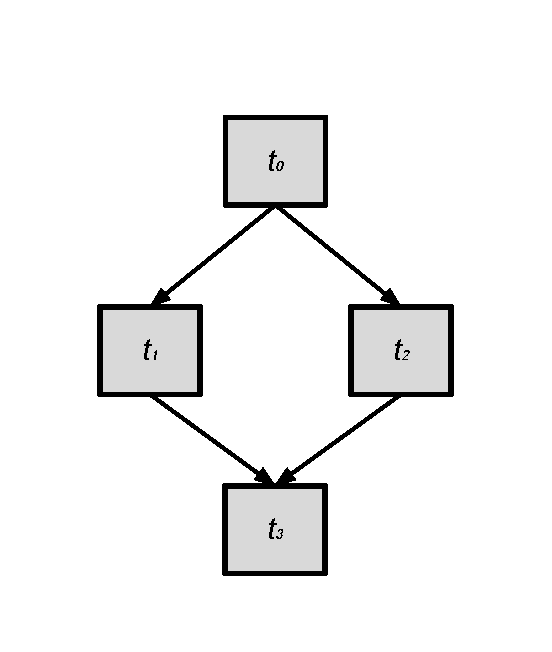
\includegraphics[width=0.3\linewidth]{figures/model/dag.pdf}
\centering
  \captionof{figure}{Simple DAG with four tasks ($t_1, t_2, t_3, t_4$). The edges represent data dependencies between tasks. }
  \label{fig:model_dag}
\end{figure}

%rewrite
Traditionally, a workflow is modeled as a Directed Acyclic Graph (DAG). As shown in Figure~\ref{fig:model_dag}, each node in the DAG represents a workflow task, and the edges represent dependencies between the tasks ($t$) that constrain the order in which the tasks are executed. Each task is a program and a set of parameters that need to be executed. The dependencies typically represent data flow dependencies in the application, where the output files produced by one task are needed as inputs of another task. 

Scientific workflows increasingly require tremendous amounts of data processing and workflows with up to a few million tasks are not uncommon \cite{Callaghan2011}. For example, the CyberShake workflow \cite{Rynge2012} composed of more than 800,000 jobs have been executed on the TeraGrid \cite{TeraGrid}. Among these large-scale, loosely-coupled applications, the majority of the tasks within these applications are often relatively small (from a few seconds to a few minutes in runtime). However, in aggregate they represent a significant amount of computation and data \cite{Deelman2002}. Most existing systems considered the allocation of computation resources and the scheduling of tasks, but did not effectively take into account the refinement of workflow structures, system overheads, and failure occurrence.
An \textbf{overhead} is defined as the time of performing miscellaneous work other than executing the user's computational activities. Overheads adversely influence runtime of large-scale scientific workflows and cause significant resource underutilization \cite{Chen2011}. 

In order to minimize the impact of system overheads, workflow restructuring techniques such as task clustering \cite{Singh2008,Hussin2010,Zhao2009} and workflow partitioning \cite{Kumar2002, Hedayat2009} have been developed to increase their computational granularity and thereby reduce the system overheads. \textbf{Task clustering}~\cite{Singh2008} is a technique that merges small tasks into larger jobs so that the number of computational activities is reduced and the ratio of application computation to the system overheads is increased. A \textbf{job} is a single execution unit in a workflow management system such as Pegasus \cite{Deelman2004}, Askalon \cite{Ostermann2009b} and Taverna \cite{Calasanz2008}. 
Figure~\ref{fig:model_system} shows a typical execution environment for scientific workflows. The components of this environment are listed below: 

\begin{figure}[h!]
\centering
  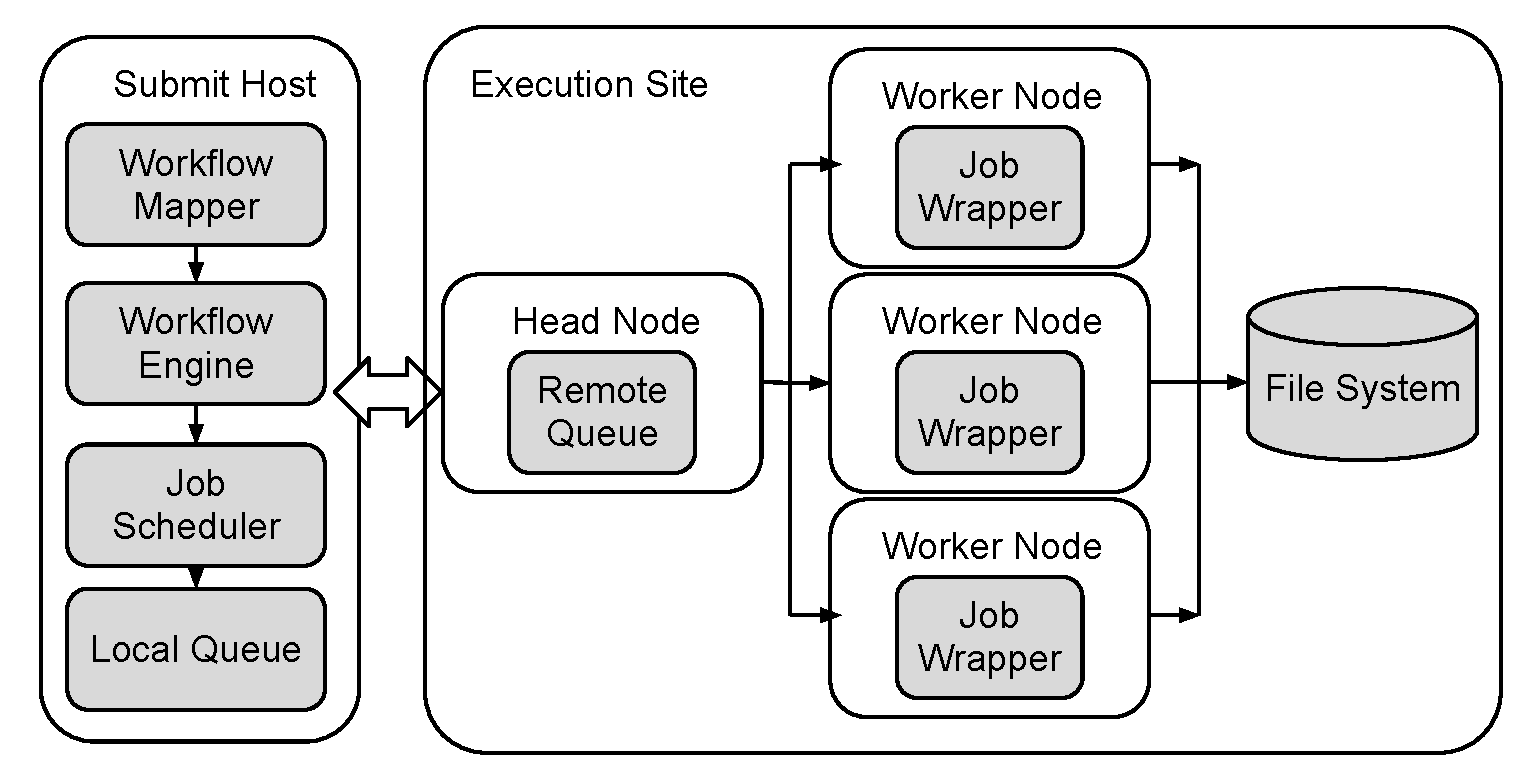
\includegraphics[width=0.7\linewidth]{figures/model/model.pdf}
  \caption{System Model}
  \label{fig:model_system}
\end{figure}

\textbf{Workflow Mapper} generates an executable workflow based on an abstract workflow provided by a user or a workflow composition system. 

\textbf{Workflow Engine} executes the jobs defined by the workflow in order of their dependencies. Only free jobs that have all their parent jobs completed are submitted to  Job Scheduler. 

\textbf{Job Scheduler} and \textbf{Local Queue} manage individual workflow jobs and supervise their execution on local and remote resources.

\textbf{Job Wrapper} extracts tasks from clustered jobs and executes them at the worker nodes. 

%Task clustering has been widely used in executing such large-scale scientific workflows and has demonstrated its great effort \cite{Singh2008}. 
\textbf{Workflow partitioning} is another technique that refines workflow structures by dividing a large workflow into several sub-workflows such that the overall number of tasks is reduced and the resource requirements of these sub-workflows can be satisfied in the execution environments. A \textbf{sub-workflow} is a workflow and also a job of a higher-level workflow. Sub-workflows are often scheduled to run in different execution sites. The performance of workflow partitioning has been evaluated in \cite{Rynge2012} and it has shown significant runtime improvement for an astronomy application. 
 
However, these existing methods are using an empirical approach to optimize the workflow structures. For example, Horizontal Clustering (HC) \cite{Singh2008} merges multiple tasks that are at the same horizontal level of the workflow. The clustering granularity (number of tasks within a cluster) of a clustered job is controlled by the user, who defines either the number of tasks per clustered job (\textit{clusters.size}), or the number of clustered jobs per horizontal level of the workflow (\textit{clusters.num}). Such an empirical approach of tuning task granularity has ignored or underestimated the dynamic characteristics of distributed environments. First of all, such a naive setting of clustering granularity may cause significant imbalance between runtime and data transfer since it heavily relies on the users' knowledge. Second, these techniques have ignored the occurrence of task failures, which can counteract the benefit from task clustering. The workflow partitioning approach~\cite{Rynge2012} has also ignored the fact that the execution environment has limited resources to host some large-scale scientific workflows, such as the data storage. 

These empirical methods have introduced many challenges for the management of large-scale scientific workflows. In next section, we generalize these drawbacks to the three research challenges. 

\section{Problem Space}

In this thesis, we identify new challenges when executing complex scientific applications in distributed environments:

The first challenge deals with the \textbf{data management within a workflow}~\cite{wang2013supporting, wang2012scimate, wang2014removing}. 
Because of the distributed nature of computational and storage resources in grids and clouds, and the fact that scientific applications usually need collaborations of scientists from different institutions, it is sometimes hard to compute where the data is. Scientists in search of compute cycles and application data are distributing computations across multiple resources. 
Thus the issue of efficient data transfers between different execution sites is becoming critical. Whenever possible, data need to be transferred in bulk with as few individual, small data transfers as possible. 
Communication-aware scheduling \cite{Sonmez2006, Jones2004} has taken the communication cost into the scheduling/clustering model and have achieved some significant improvement. The workflow partitioning approach \cite{Hedayat2009, Yuan2010, Wieczorek2005,Rubing2005} represents the partitioning problem as a global optimization problem and aims to minimize the overall runtime of a graph. However, the complexity of solving such an optimization problem does not scale well. Heuristics \cite{Maheshwari2012, Callaghan2010} are used to select the right parameters and achieve better runtime performance but the approach is not automatic and requires much knowledge in applications. 


The second challenge deals with the \textbf{imbalance of runtime and data dependency} when merging workflow tasks. Tasks may have diverse runtimes and such diversity may cause significant load imbalance. To address this challenge, researchers have proposed several approaches. Bag-of-Tasks \cite{Hussin2010, Celaya2010, Oprescu2010} dynamically groups tasks together based on the task characteristics but it assumes tasks are independent, which limits its usage in scientific workflows. Singh \cite{Singh2008} and Rynge \cite{Rynge2012} examine the workflow structures and group tasks together into jobs in a static way for Pegasus Workflow Management Systems~\cite{Deelman2004}.
However, this work ignores the computational requirements of tasks and may result in an imbalanced load on the resources. A popular technique in workload studies to address the load balancing challenge is over-decomposition \cite{Lifflander2012}. This method decomposes computational work into medium-grained tasks. Each task is coarse-grained enough to enable efficient execution and to reduce scheduling overheads, while being fine-grained enough to expose significantly higher application-level parallelism than that is offered by the hardware. 

%However, what makes this problem even challenging is that solutions to address the data dependency challenge usually conflicts Therefore, we claim that it is necessary to consider the data dependencies with subsequent tasks (not only child tasks). However, they have forgotten balance and data structure problem. 


%\textbf{Resource management} is the third challenge that is brought by the recent emergence of cloud computing and resource provisioning techniques. Along with the increase of the scale of workflows, the number and the variety of computational resources to use has been increasing consistently. Infrastructure-as-a-Service (IaaS) clouds offer the ability to provision resources on-demand according to a pay-per-use model and adjust resource capacity according to the changing demands of the application \cite{Abrishami2012}. Task clustering can still be applied to this cloud scenario \cite{Deelman2010, Vockler2011}. However, the decisions required in cloud scenarios not only have to take into account performance-related metrics such as workflow makespan, but must also consider the resource utilization, since the resources from commercial clouds usually have monetary costs associated with them. Therefore, the adoption of task clustering on cloud computing requires the development of new methods for the integration of task clustering and resource provisioning. 

%Fault Tolerance Challenge
The third challenge deals with \textbf{fault tolerance}. Existing clustering strategies ignore or underestimate the influence of the occurrence of failures on system behavior, despite the fact that failures are commonplace in large-scale distributed systems. Many researchers \cite{Zhang2004, Tang1990, Schroeder2006, Sahoo2004} have emphasized the importance of fault tolerance design and indicated that the failure rates in modern distributed systems are significant. The major concern has to do with transient failures because they are expected to be more prevalent than permanent failures \cite{Zhang2004}. For example, denser integration of semiconductor circuits and lower operating voltage levels may increase the likelihood of bit-flips when circuits are bombarded by cosmic rays and other particles \cite{Zhang2004}. In a faulty environment, there are usually three approaches for managing workflow failures. First, one can simply retry the entire job when its computation is not successful as in the Pegasus Workflow Management System~\cite{Deelman2004}. However, some of the tasks within the job may have completed successfully and it could be a waste of time and resources to retry all of the tasks. Second, the application process can be periodically check-pointed so that when a failure occurs, the amount of work to be retried is limited. However, the overheads of checkpointing can limit its benefits \cite{Zhang2004}. Third, tasks can be replicated to different nodes to avoid location-specific failures \cite{Zhang2009}. However, this approach increases resource cost since it has duplicate tasks. 
%Intuitively, a long-running job that consists of many tasks has a higher job failure rate even when the overall task failure rate is low. 


% After examining the major challenges in executing large-scale scientific workflows, we contribute to the studies of workflow performance improvement through task clustering in the following aspects:


\section{Thesis Statement}
This thesis states that \textbf{refining workflow structures can significantly improve the runtime performance of executing scientific workflows in distributed environments}. We distinguish our work from prior work in the following way: First, we propose data aware workflow partitioning to divide large workflows into sub-workflows that satisfy the data storage limit in the execution environments. Second, we propose a series of balanced task clustering strategies to address the tradeoff between the dependency imbalance and the runtime imbalance. Third, we propose fault tolerant clustering algorithms to automatically adjust the task granularity in a faulty execution environment and thereby improve the overall runtime of executing scientific workflows. 

This thesis uses a wide range of scientific workflows to demonstrate the efficiency and effectiveness of our approaches. 
%We believe our contributions of new task clustering and workflow partitioning mechanism and knowledge can be used by future workflow management systems to overcome resource constraints, load imbalance and improve fault tolerance. 
We believe that our methods can be used by many domain scientists to optimize their scientific workflows and will inspire new ways for future optimization of runtime performance in scientific workflows. 


%This thesis states that \textbf{optimization in task granularity is necessary for large-scale scientific workflows in modern distributed environments}.  First, we build an overhead and workflow model to demonstrate the reason why and how scientific workflows benefits from task clustering. Second, we develop resource aware heuristics to partition large-scale workflows into sub-workflows to satisfy resource constraints. Third, we develop a series of effective balancing algorithms to address the tradeoff of dependency imbalance and runtime imbalance. Last, we develop an effective transient failure model to study the influence of failure occurrence on task clustering to further improve the performance of task clustering in a faulty environment. This thesis use a wide range of scientific workflows to demonstrate the efficiency and effectiveness of our approaches. We believe our contributions of new task clustering mechanism and knowledge can be used by future workflow management systems to overcome resource constraints, load imbalance and improve fault tolerance. 

\section{Supporting the Thesis Statement}

In this section, we substantiate the thesis statement through four specific studies, each gaining new insights and knowledge about the optimization of task granularity in scientific workflows. 

In our first work \cite{Chen2011} (Chapter \ref{chap:model}), we \textbf{extend the existing Directed Acyclic Graph (DAG) model to be overhead-aware} and analyze the relationship between the workflow performance and overheads. Previous research has established models to describe system overheads in distributed systems and has classified them into several categories \cite{Prodan2007, Prodan2008}. In contrast, we investigate the distributions and patterns of different overheads and discuss how the system environment (system configuration, etc.) influences the distribution of overheads. Furthermore, we have developed a workflow simulator based on our overhead-aware DAG model and evaluated its effectiveness. 
%Furthermore, we present quantitative metrics to measure and evaluate the characters (robustness, sensitivity, balance, etc.) of workflows. Finally, we analyze the relationship between these metrics and the workflow performance with different optimization methods. 

In our second work \cite{Integration2012, Chen2011a} (Chapter \ref{chap:partitioning}), we introduce \textbf{data aware workflow partitioning} to refine workflow structures and data management within large-scale scientific workflows. Data-intensive workflows require significant amount of storage and computation. For these workflows, we need to use multiple execution sites and consider their available storage. Data aware partitioning aims to reduce the intermediate data transfer in a workflow while satisfying the storage constraints. Heuristics and algorithms are proposed to improve the efficiency of partitioning. Experiment-based evaluation is performed to validate its effectiveness.  

In our third work \cite{Chen2013a,Chen2013b} (Chapter \ref{chap:balance}), we \textbf{solve the runtime and data dependency imbalance problem} and introduce a series of balanced clustering methods. 
%The imbalance problem means that the execution of workflows suffers from significant overheads (unavailable data, overloaded resources, or system constraints) due to inefficient task clustering and job execution. 
We identify the two challenges: runtime imbalance due to the inefficient clustering of independent tasks and dependency imbalance that is related to dependent tasks. What makes this problem even more challenging is that solutions to address these two problems are usually conflicting. For example, balancing runtime may aggravate the dependency imbalance problem, and vice versa. A quantitative measurement of workflow characteristics is required to serve as a criterion to select and balance these solutions. To achieve this goal, we propose a series of imbalance metrics to reflect the internal structure (in terms of runtime and dependency) of the workflow. 

In our fourth work \cite{Chen2012} (Chapter \ref{chap:tolerance}), we propose \textbf{fault tolerant clustering} techniques that dynamically adjusts the clustering strategy based on the current trend of failures. During the runtime, this approach uses Maximum Likelihood Estimation to estimate the failure distribution among all the resources. We then dynamically merge tasks into jobs of moderate size and recluster failed jobs to avoid further failures.


Overall, this thesis aims to \textbf{improve the quality of task clustering and workflow partitioning methods in large-scale scientific workflows}. We present both experiment-based and simulation-based evaluation of our algorithms on a wide range of scientific workflows. 


\section{Research Contributions}

The main contribution of this thesis is a framework for task clustering and workflow partitioning in executing scientific workflows. Specially, 
\begin{enumerate}
\item We developed an overhead-aware workflow model to investigate the performance of task clustering techniques in distributed environments. We present the overhead characteristics for a wide range of widely used workflows.
% In addition, we have showed how existing workflow optimization methods improve runtime performance by reducing some or all types of overheads.
\item We have developed workflow partitioning algorithms that use heuristics to divide large-scale workflows into sub-workflows to satisfy resource constraints at execution sites such as data storage constraint. 
\item We have built a statistical model to demonstrate that transient failures can have a significant impact on the runtime of scientific workflows. We have developed a Maximum Likelihood Estimation based parameter estimation approach to integrate both prior knowledge and runtime feedbacks about task runtime, system overheads and transient failures. We have proposed fault tolerant clustering algorithms to dynamically adjust the task granularity and improve the runtime. 
\item We have examined the reasons that cause runtime imbalance and dependency imbalance in task clustering. We have proposed quantitative metrics to evaluate the severity of the two imbalance problems and a series of balanced clustering methods to address the imbalance problems for five widely used scientific workflows. 
\item We have developed an innovative workflow simulator called WorkflowSim that includes popular task scheduling and task clustering algorithms. 
We have built an open source community for the users and developers of WorkflowSim. Furthermore, our balanced algorithms have been implemented in the Pegasus Workflow Management Systems~\cite{Deelman2014}. 
%\item Using a set of trace-based simulations, we compare the overall performance with existing approaches for a wide range of popular scientific workflows. We show that the proposed approach can provide significant improvement for the application. 
\end{enumerate}
 
%In particular, we provide a novel approach to capture these metrics. Our work considers the neighboring tasks including siblings, parents, children and so on because such a family of tasks has strong connections between them. The performance evaluation shows that they can significantly reduce the imbalance problem and we analyze and connect the performance of these metrics and balancing methods. These quantitative metrics indicate which type of imbalance problem a workflow is more likely to suffer from. Comparing the relative values of these metrics informs the selection of a balancing method or a combination of these methods. 

%The Pegasus Workflow Management System (Pegasus WMS) is a framework for mapping complex workflows onto distributed resources such as grids and clouds. Pegasus has been used to optimize runtime performance of various scientific applications in astronomy, biology, physics, and earthquake science on dedicated clusters, and national cyberinfrastructure such as the TeraGrid and the Open Science Grid. To prepare and execute a large-scale workflows on these distributed environments has features such as the distributed nature of these resources, the large number of tasks in a workflow, and the complex dependencies among the tasks. Due to these features, significant overheads can occur during workflow execution. Failures occurring to different layers of the workflow management systems may exist. These challenges are hard to solved with conventional scheduling algorithm based approach. Instead, we aim to use a workflow restructuring approach that reorganizes workflow activities within it to improve the resource utilization, runtime performance and fault tolerance. For example, many of existing algorithms have ignored or underestimated the overheads and runtimes variabilities. 

